\documentclass[11pt,a4paper]{article}

% ---------------------------------------------------------------- packages
\usepackage[utf8]{inputenc}
\IfFileExists{lmodern.sty}{\usepackage[T1]{fontenc}\usepackage{lmodern}}{}
\usepackage[english]{babel}
\usepackage[a4paper,margin=2.5cm]{geometry}
\usepackage{microtype}
\usepackage{amsmath,amssymb}
\usepackage{graphicx}
\usepackage{booktabs}
\usepackage[font=small,labelfont=bf,skip=6pt]{caption}
\usepackage{subcaption}
\usepackage[round,authoryear]{natbib}
\usepackage{xcolor}
\definecolor{linkblue}{HTML}{1F5FAD}
\usepackage[colorlinks=true,linkcolor=linkblue,citecolor=linkblue,urlcolor=linkblue]{hyperref}
\usepackage{titlesec}
\titleformat{\section}{\large\bfseries}{\thesection}{0.6em}{}
\titleformat{\subsection}{\normalsize\bfseries}{\thesubsection}{0.6em}{}
\titlespacing*{\section}{0pt}{14pt}{6pt}
\titlespacing*{\subsection}{0pt}{10pt}{4pt}
\setlength{\parskip}{3pt}

\newcommand{\dV}{\Delta V}
\newcommand{\dA}{\Delta A}
\newcommand{\dD}{\Delta D}

% ---------------------------------------------------------------- title
\title{\vspace{-1.2cm}\textbf{How Does Language Organize Emotions?}\\[4pt]
\large Distributional Semantics Meets Valence, Arousal and Dominance Norms}
\author{Nathan Tessot\\[2pt]
\small CPES -- Data Science \& Cultural Sciences, Université PSL\\
\small Computational linguistics project\\[2pt]
\small \href{https://github.com/NathanTessot75/emotions-language}{\texttt{github.com/NathanTessot75/emotions-language}}}
\date{\small May 2026}

\begin{document}
\maketitle

% ---------------------------------------------------------------- abstract
\begin{abstract}
\noindent
Do emotion words that are used in similar linguistic contexts also share
similar psychological properties? I compare two independent representations
of 53 English emotion words: Word2Vec embeddings trained on Google News,
which capture how words are used, and the valence--arousal--dominance (VAD)
ratings of \citet{warriner2013}, which capture how they are experienced.
Pairs of emotions whose embeddings are similar (cosine $\geq 0.50$) are
markedly closer in VAD space than other pairs (mean Euclidean distance 2.26
vs.\ 3.63; Welch's $t = -7.58$, $p < 10^{-11}$), a result that survives a
permutation test respecting the dependence between pairs ($p < 10^{-4}$).
A logistic regression on the three per-axis differences shows that valence
and dominance each predict semantic proximity, with effects of almost equal
size once standardized, while arousal has no detectable effect. Contrary
to my initial hypothesis, valence is therefore not the only dimension that
structures emotional vocabulary: the sense of control an emotion conveys
matters as much.
\end{abstract}

% ---------------------------------------------------------------- 1
\section{Introduction}

When we think about emotions, we spontaneously group some of them together:
\emph{joy} and \emph{happiness} feel related, while \emph{joy} and
\emph{anger} feel like opposites. Psychologists have long proposed that this
intuition can be described with a small number of affective dimensions.
Following the semantic differential of \citet{osgood1957} and the
pleasure--arousal--dominance model of \citet{mehrabian1974}, three dimensions
have become standard: \emph{valence} (negative to positive), \emph{arousal}
(calm to excited) and \emph{dominance} (overwhelmed to in control).
\citet{warriner2013} collected such ratings for almost 14{,}000 English
lemmas.

Computational linguistics offers a very different route to word meaning.
Following the distributional hypothesis \citep{harris1954}, models such as
Word2Vec \citep{mikolov2013a,mikolov2013b} learn a vector for each word from
the contexts in which it appears, without any human labelling. Two words
used in similar contexts end up with similar vectors.

These two representations are built from entirely different data: one from
introspective judgements, the other from co-occurrence statistics in news
text. Comparing them asks whether the way we \emph{use} emotion words
already encodes how we \emph{experience} the emotions they name, and if so,
along which dimensions. My hypothesis was that valence, the most salient
affective dimension \citep{russell1980}, would be the main organizing
factor, with arousal and dominance playing a minor role.

% ---------------------------------------------------------------- 2
\section{Data and methods}

\subsection{Emotion words and VAD norms}

I selected 53 common English emotion words spanning basic emotions
(\emph{anger}, \emph{fear}, \emph{joy}) and more complex ones
(\emph{compassion}, \emph{embarrassment}, \emph{gratitude}), together with a
few general evaluative terms (\emph{good}, \emph{bad}). All 53 appear in the
\citet{warriner2013} norms, from which I take the mean valence, arousal and
dominance ratings (each on a 1--9 scale). Figure~\ref{fig:dist} shows their
distribution. Valence is strongly bimodal, separating negative from positive
emotions, whereas arousal is concentrated in the middle of the scale.

\begin{figure}[h]
  \centering
  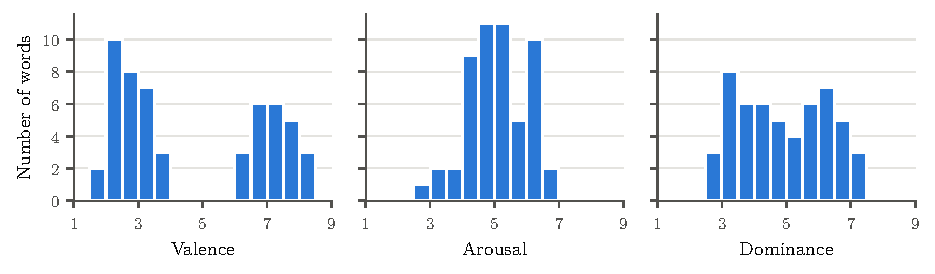
\includegraphics[width=\linewidth]{figures/fig1_vad_distributions.pdf}
  \caption{Distribution of the VAD ratings of the 53 emotion words
  \citep{warriner2013}.}
  \label{fig:dist}
\end{figure}

\subsection{Semantic links from Word2Vec}

For every pair of words I computed the cosine similarity of their
300-dimensional Word2Vec vectors (Google News model). A pair is considered
\emph{semantically linked} if its similarity is at least 0.50. Similarities
between related words typically fall between 0.3 and 0.7 in this model, and
0.50 retains clearly related pairs without being overly restrictive. This
yields 89 links. Five words have no link at this threshold
(\emph{awe}, \emph{contempt}, \emph{relief}, \emph{terror}, \emph{want}) and
are excluded, leaving 48 words and $\binom{48}{2} = 1{,}128$ pairs, of which
7.9\% are linked.

\subsection{Statistical analysis}

For each pair $(i,j)$ I compute the absolute differences on each axis,
$\dV$, $\dA$ and $\dD$, and the Euclidean distance
$d_{ij} = \sqrt{\dV^2 + \dA^2 + \dD^2}$ in VAD space. Two questions are
then asked.

\begin{enumerate}
  \item \textbf{Are linked pairs closer in VAD space?} I compare the mean
  distance of linked and unlinked pairs with Welch's $t$-test. Because each
  word appears in 47 pairs, pairs are not independent. As a robustness
  check, I therefore also run a permutation test in the spirit of the
  quadratic assignment procedure \citep{krackhardt1988}: the VAD profiles
  are randomly reassigned to words 10{,}000 times while the network of links
  is held fixed, and the observed difference in mean distance is compared
  with this null distribution.
  \item \textbf{Which dimensions matter?} I fit a logistic regression
  predicting the binary link status from $\dV$, $\dA$ and $\dD$. Since the
  three differences have different spreads (standard deviations of 2.07,
  0.78 and 1.12), I also report coefficients for standardized predictors,
  which make the effects directly comparable.
\end{enumerate}

% ---------------------------------------------------------------- 3
\section{Results}

\subsection{The semantic network in affective space}

Figure~\ref{fig:network} projects the 48 words onto the two dimensions that
turn out to matter, valence and dominance, and draws the 89 semantic links.
Two dense clusters appear: a low-valence, low-dominance cluster
(\emph{anxiety}, \emph{fear}, \emph{grief}, \emph{frustration},
\emph{panic}) and a high-valence, high-dominance cluster (\emph{joy},
\emph{happiness}, \emph{optimism}, \emph{contentment}). Most links (70 of
89) connect two words on the same side of the valence midpoint. Many of the
long links crossing the valence axis connect antonyms, such as
\emph{love}--\emph{hate}, \emph{good}--\emph{bad} or
\emph{joy}--\emph{sadness}, which Word2Vec is known to place close
together because they appear in the same contexts.

\begin{figure}[t]
  \centering
  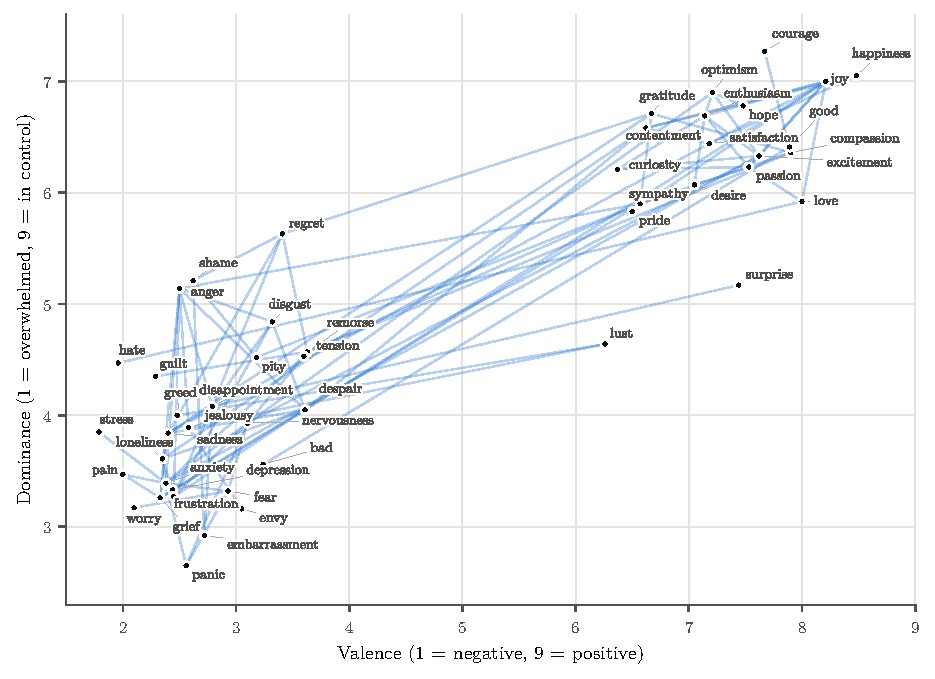
\includegraphics[width=\linewidth]{figures/fig2_network_vd.pdf}
  \caption{The 48 linked emotion words placed by valence and dominance
  \citep{warriner2013}. Lines connect pairs whose Word2Vec cosine similarity
  is at least 0.50 (89 links). Arousal, the third dimension, is not shown.}
  \label{fig:network}
\end{figure}

\subsection{Linked emotions are psychologically closer}

Linked pairs are substantially closer in VAD space than unlinked pairs
(Table~\ref{tab:ttest}, Figure~\ref{fig:box}). The mean distance drops from
3.63 to 2.26 and the median from 3.80 to 1.75, a difference of about
0.7 pooled standard deviations. Welch's test gives $t(114) = -7.58$,
$p = 9.9 \times 10^{-12}$. The permutation test confirms the result: none of
the 10{,}000 random reassignments produced a difference as large as the one
observed ($p < 10^{-4}$), so the effect is not an artefact of the dependence
between pairs.

\begin{table}[h]
  \centering
  \small
  \begin{tabular}{lrrrr}
    \toprule
    Pairs & $n$ & Mean distance & SD & Median \\
    \midrule
    Linked     &    89 & 2.26 & 1.60 & 1.75 \\
    Not linked & 1{,}039 & 3.63 & 2.04 & 3.80 \\
    \bottomrule
  \end{tabular}
  \caption{Euclidean distance in VAD space by semantic link status. Welch's
  $t(114) = -7.58$, $p < 10^{-11}$; permutation test (10{,}000 draws):
  $p < 10^{-4}$.}
  \label{tab:ttest}
\end{table}

\begin{figure}[h]
  \centering
  \begin{subfigure}[b]{0.50\linewidth}
    \centering
    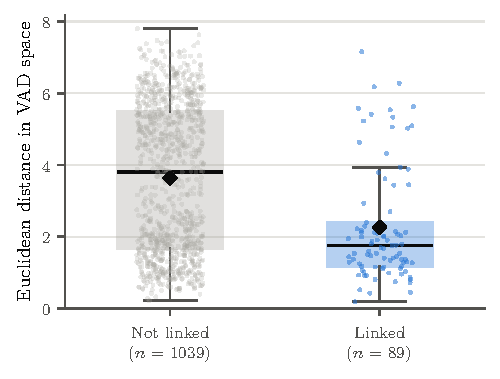
\includegraphics[width=\linewidth]{figures/fig3_distance_boxplot.pdf}
    \caption{VAD distance by link status. Diamonds mark the means.}
    \label{fig:box}
  \end{subfigure}\hfill
  \begin{subfigure}[b]{0.46\linewidth}
    \centering
    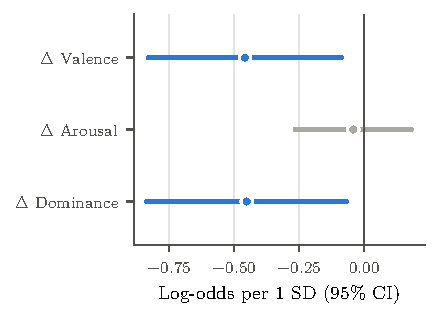
\includegraphics[width=\linewidth]{figures/fig4_coefficients.pdf}
    \caption{Standardized logistic regression coefficients.}
    \label{fig:coef}
  \end{subfigure}
  \caption{Main results. Grey marks a non-significant effect.}
\end{figure}

\subsection{Valence and dominance, not arousal}

Table~\ref{tab:logit} reports the logistic regression. Differences in
valence ($p = 0.016$) and dominance ($p = 0.021$) both significantly lower
the probability that two emotions are semantically linked, while the
difference in arousal has no detectable effect ($p = 0.72$). The model as a
whole is highly significant (likelihood-ratio $p = 2.6 \times 10^{-9}$),
although its modest pseudo-$R^2$ (0.07) shows that VAD differences explain
only part of the semantic structure.

In raw units, the dominance coefficient ($-0.40$) is about twice the valence
coefficient ($-0.22$). This comparison is misleading, however, because a
one-point difference in dominance is rarer than a one-point difference in
valence. With standardized predictors (Figure~\ref{fig:coef}), the two
effects are almost identical: one standard deviation of additional distance
reduces the odds of a link by 37\% for valence ($\beta = -0.46$) and by
36\% for dominance ($\beta = -0.45$). The two predictors are also strongly
correlated ($r = 0.75$ between $\dV$ and $\dD$), as positive emotions tend to
be felt as controllable. Their separate contributions should therefore be
read as roughly equal rather than ranked.

\begin{table}[h]
  \centering
  \small
  \begin{tabular}{lrrrrrr}
    \toprule
    & $\beta$ & SE & $z$ & $p$ & Odds ratio & $\beta_{\text{std}}$ \\
    \midrule
    Intercept         & $-1.458$ & 0.230 & $-6.34$ & $<0.001$ & --    & --        \\
    $\dV$ (valence)   & $-0.221$ & 0.091 & $-2.42$ & 0.016    & 0.80  & $-0.458$  \\
    $\dA$ (arousal)   & $-0.052$ & 0.146 & $-0.36$ & 0.720    & 0.95  & $-0.041$  \\
    $\dD$ (dominance) & $-0.403$ & 0.175 & $-2.30$ & 0.021    & 0.67  & $-0.451$  \\
    \midrule
    \multicolumn{7}{l}{$N = 1{,}128$ pairs; McFadden pseudo-$R^2 = 0.069$;
    LR test $p = 2.6 \times 10^{-9}$} \\
    \bottomrule
  \end{tabular}
  \caption{Logistic regression of semantic link status on absolute VAD
  differences. Odds ratios are per one-point difference on the 1--9 scale;
  $\beta_{\text{std}}$ is the coefficient per standard deviation.}
  \label{tab:logit}
\end{table}

% ---------------------------------------------------------------- 4
\section{Discussion}

The way emotion words are distributed in news text does reflect how people
rate the corresponding emotions. Emotions that are used in similar contexts
are, on average, close in affective space, and this proximity is carried by
two dimensions. Valence is one of them, as expected. The surprise is
dominance: whether an emotion makes us feel in control (\emph{pride},
\emph{courage}) or overwhelmed (\emph{panic}, \emph{embarrassment}) shapes
its linguistic neighbourhood as much as whether it is pleasant. My initial
hypothesis that valence alone organizes emotional vocabulary is therefore
only partly supported.

The absence of an arousal effect is also informative. Emotions of very
different intensity are often linked: \emph{grief} and \emph{sadness},
\emph{happiness} and \emph{satisfaction}, or \emph{enthusiasm} and
\emph{excitement} are close in usage despite arousal gaps of two to three
points. One
interpretation is that language groups emotions by \emph{what kind} of
situation they evaluate rather than by \emph{how strongly} they are felt,
intensity being expressed by other means (adverbs, intensifiers, word
choice within a family).

\subsection*{Limitations}

\begin{itemize}
  \item \textbf{Language and population.} The study covers English only, and
  the VAD ratings come from a single, mainly American sample. Emotional
  vocabulary may be organized differently in other languages and cultures.
  \item \textbf{Word selection.} The 53 words were chosen manually, and five
  of them had no link at the chosen threshold. A different list, or a
  lexicon-driven selection, could change the results.
  \item \textbf{Threshold.} Links are defined by a single cosine cut-off
  (0.50). Testing the robustness of the results across thresholds, or
  modelling the similarity as a continuous variable, would strengthen the
  conclusions.
  \item \textbf{Embeddings.} Static Word2Vec vectors conflate senses and
  place antonyms close together. Contextual embeddings, or a corpus other
  than news, may give a different picture.
  \item \textbf{Dependence between pairs.} The permutation test addresses
  this for the distance comparison, but the standard errors of the logistic
  regression assume independent observations and are likely too small.
\end{itemize}

% ---------------------------------------------------------------- 5
\section{Conclusion}

Comparing distributional and psychological representations of 53 emotion
words shows that linguistic usage and affective experience are aligned:
semantically related emotions are closer in VAD space. This alignment runs
along valence and dominance in roughly equal measure, not along arousal.
Emotional vocabulary is therefore organized not only by how good or bad an
emotion feels, but also by how much control it grants us.

\medskip
\noindent\textbf{Code and data.} The analysis was carried out in Python
(pandas, gensim, SciPy, statsmodels). The notebook, the data and the scripts
reproducing every figure and statistic of this report are available at:
\begin{center}
\small\url{https://github.com/NathanTessot75/emotions-language}
\end{center}

% ---------------------------------------------------------------- refs
\begin{thebibliography}{99}
\setlength{\itemsep}{1pt}\small

\bibitem[Harris(1954)]{harris1954}
Harris, Z.~S. (1954). Distributional structure. \emph{Word}, 10(2--3),
146--162.

\bibitem[Krackhardt(1988)]{krackhardt1988}
Krackhardt, D. (1988). Predicting with networks: Nonparametric multiple
regression analysis of dyadic data. \emph{Social Networks}, 10(4), 359--381.

\bibitem[Mehrabian and Russell(1974)]{mehrabian1974}
Mehrabian, A., \& Russell, J.~A. (1974). \emph{An Approach to Environmental
Psychology}. MIT Press.

\bibitem[Mikolov et~al.(2013a)]{mikolov2013a}
Mikolov, T., Chen, K., Corrado, G., \& Dean, J. (2013a). Efficient
estimation of word representations in vector space. \emph{arXiv preprint}
arXiv:1301.3781. \url{https://arxiv.org/abs/1301.3781}

\bibitem[Mikolov et~al.(2013b)]{mikolov2013b}
Mikolov, T., Sutskever, I., Chen, K., Corrado, G., \& Dean, J. (2013b).
Distributed representations of words and phrases and their
compositionality. In \emph{Advances in Neural Information Processing
Systems 26}.

\bibitem[Osgood et~al.(1957)]{osgood1957}
Osgood, C.~E., Suci, G.~J., \& Tannenbaum, P.~H. (1957). \emph{The
Measurement of Meaning}. University of Illinois Press.

\bibitem[Russell(1980)]{russell1980}
Russell, J.~A. (1980). A circumplex model of affect. \emph{Journal of
Personality and Social Psychology}, 39(6), 1161--1178.

\bibitem[Warriner et~al.(2013)]{warriner2013}
Warriner, A.~B., Kuperman, V., \& Brysbaert, M. (2013). Norms of valence,
arousal, and dominance for 13,915 English lemmas. \emph{Behavior Research
Methods}, 45(4), 1191--1207. \url{https://doi.org/10.3758/s13428-012-0314-x}

\end{thebibliography}

\end{document}
